\section{Evaluation}

\subsection{Experimental setup}
\textbf{Hardware.} Cross-device measurements were performed on two configurations representing the hardware spectrum that students typically use:
\begin{itemize}[leftmargin=1.4em]
    \item \textit{Laptop tier (mid-range gaming laptop):} ASUS TUF Gaming F15 (FX506HC), Intel Core i5-11400H @ 4.10 GHz (6 cores / 12 threads), 16 GB DDR4-3200 RAM, NVIDIA GeForce RTX 3050 Laptop GPU (4 GB VRAM), Windows 11 Home.

    \item \textit{Desktop tier (mid-range workstation):} Intel Core i7-8700K @ 4.70 GHz (6 cores / 12 threads), 32 GB DDR4-3200 RAM, NVIDIA GeForce GTX 1080 (8 GB VRAM), MSI Z390-A Pro motherboard, Windows 10 Pro.
\end{itemize}
The browser was Microsoft Edge 147.0.3912.86 with hardware acceleration enabled on both systems. Display resolution was fixed at 1920$\times$1080 with devicePixelRatio = 1.0. Each test was preceded by a 10-second idle period to allow background browser processes to settle.

\textbf{Benchmark scenes.}
\begin{itemize}[leftmargin=1.4em]
    \item \textit{Scene 1 -- Procedural primitives grid.} A grid of $N$ primitive geometries with shared meshes and materials, $N \in \{100, 500, 1000, 5000\}$, of which 5\% rotate every frame. Isolates per-frame transform overhead.
    \item \textit{Scene 2 -- High-polygon textured model.} A single PBR-textured 3D model with 218{,}400 vertices, 436{,}810 triangles, and 4 textures (4K base color, normal, roughness, ambient occlusion).
    \item \textit{Scene 3 -- Solar System educational scenario.} The complete educational scenario as deployed in the platform: six PBR-textured planets, sun with point lighting, equirectangular skybox, planetary orbits, and a Cinemachine-based camera rig (15 draw calls, 37{,}132 triangles, 14 textures, 7 shader programs, 21 GameObjects).
\end{itemize}

\textbf{Metrics.} Loading time; mean, median, p95, p99, and maximum frame time over a 600-frame sample after a 120-frame warmup; JavaScript heap usage; Three.js renderer info.

\textbf{Repetition protocol.} Each Scene 1 and Scene 2 configuration was executed three times; each Scene 3 configuration ten times. Reported values are mean $\pm$ standard deviation.

\subsection{Scene 1 -- Per-frame transform overhead}
Table~\ref{tab:scene1} reports average frame time as a function of object count for Scene 1, with and without dirty-flag transforms enabled.

\begin{table}[H]
\centering
\caption{Scene 1 -- Average frame time (ms) on the laptop tier.}
\label{tab:scene1}
\begin{tabular}{lccc}
\toprule
Objects & Dirty OFF (ms) & Dirty ON (ms) & Reduction \\
\midrule
100  & 7.03 $\pm$ 0.81 & 6.96 $\pm$ 0.58 & -1.0\% \\
500  & 8.24 $\pm$ 1.49 & 8.26 $\pm$ 1.06 & +0.2\% \\
1000 & 9.11 $\pm$ 1.33 & 9.10 $\pm$ 0.92 & -0.1\% \\
5000 & 21.61 $\pm$ 0.93 & 20.24 $\pm$ 1.12 & -6.3\% \\
\bottomrule
\end{tabular}
\end{table}

The optimization produces a measurable reduction only at 5000 objects, confirming the design intent: the dirty-flag mechanism targets large scenes with predominantly static objects. For educational scenarios with smaller object counts, the optimization adds no measurable benefit but also no measurable cost.

\subsection{Scene 2 -- High-polygon model rendering}
Across all configurations of texture maxSize and shader warmup, the engine sustained an average frame time between 9.97 and 10.96 ms on the laptop tier (approximately 95--100 FPS). Loading time was dominated by GLB decoding (~900 ms). The scene contains only four textures and one material, so neither texture downscaling nor shader pre-compilation produced visible improvements in this configuration. The result establishes that the engine sustains stable interactive frame rates on high-polygon geometry.

\subsection{Scene 3 -- Incremental optimization stack on the laptop tier}
Table~\ref{tab:scene3-laptop} reports the metrics for each configuration as optimizations are added incrementally on the laptop tier.

\begin{table}[H]
\centering
\small
\setlength{\tabcolsep}{3pt}
\caption{Scene 3 (Solar System) on laptop tier -- Incremental impact of optimizations. Mean $\pm$ std. dev. over 10 runs.}
\label{tab:scene3-laptop}

\begin{tabularx}{\textwidth}{@{}c>{\raggedright\arraybackslash}Xrrrrrr@{}}
\toprule
\# &
\makecell[l]{Configuration} &
\makecell{Load\\(ms)} &
\makecell{Avg frame\\(ms)} &
\makecell{p99\\(ms)} &
\makecell{Max\\(ms)} &
FPS &
\makecell{Heap\\(MB)} \\
\midrule

3.1 & Baseline & 164 $\pm$ 27 & 9.07 $\pm$ 0.46 & 15.78 & 37.6 $\pm$ 33.0 & 110.5 & 40.3 $\pm$ 4.4 \\
3.2 & + textureMaxSize=2048 & 386 $\pm$ 18 & 8.47 $\pm$ 0.17 & 12.53 & 18.0 $\pm$ 9.9 & 118.1 & 42.9 $\pm$ 3.2 \\
3.3 & + releaseArchive & 376 $\pm$ 19 & 8.59 $\pm$ 0.25 & 13.89 & 16.6 $\pm$ 2.0 & 116.6 & 39.8 $\pm$ 3.1 \\
3.4 & + releaseSourceImages & 386 $\pm$ 12 & 8.36 $\pm$ 0.13 & 12.96 & 15.6 $\pm$ 2.1 & 119.6 & 45.0 $\pm$ 2.5 \\
3.5 & + KTX2 textures & 826 $\pm$ 75 & 8.32 $\pm$ 0.11 & 11.81 & 15.5 $\pm$ 1.9 & 120.3 & 67.9 $\pm$ 2.3 \\
3.6 & + shader warmup & 837 $\pm$ 73 & 8.32 $\pm$ 0.03 & 12.00 & 15.2 $\pm$ 1.0 & 120.2 & 68.7 $\pm$ 2.9 \\
3.7 & + dirty transforms (full stack) & 824 $\pm$ 64 & 8.34 $\pm$ 0.09 & 11.83 & 15.0 $\pm$ 0.8 & 119.9 & 66.7 $\pm$ 1.8 \\
\bottomrule
\end{tabularx}
\end{table}

Figure~\ref{fig:incremental} visualizes the incremental progression of the maximum frame time across the seven configurations of Table~\ref{tab:scene3-laptop}.

\begin{figure}[h]
\centering
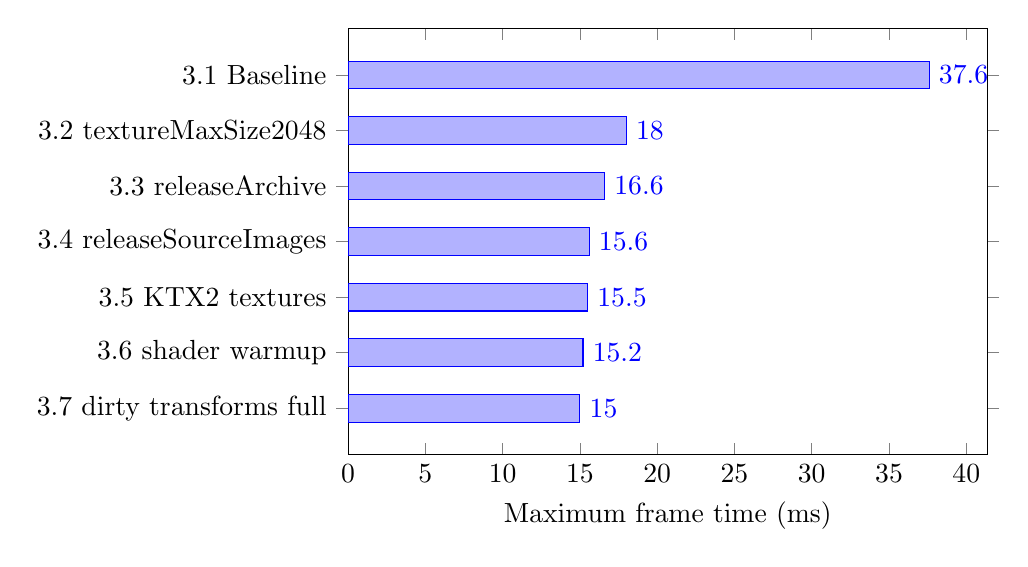
\begin{tikzpicture}
\begin{axis}[
    xbar,
    width=0.8\linewidth,
    height=7cm,
    xmin=0,
    xlabel={Maximum frame time (ms)},
    symbolic y coords={
        3.1 Baseline,
        3.2 textureMaxSize2048,
        3.3 releaseArchive,
        3.4 releaseSourceImages,
        3.5 KTX2 textures,
        3.6 shader warmup,
        3.7 dirty transforms full
    },
    ytick=data,
    y dir=reverse,
    nodes near coords,
    enlarge y limits=0.14,
]
\addplot coordinates {
    (37.6,3.1 Baseline)
    (18.0,3.2 textureMaxSize2048)
    (16.6,3.3 releaseArchive)
    (15.6,3.4 releaseSourceImages)
    (15.5,3.5 KTX2 textures)
    (15.2,3.6 shader warmup)
    (15.0,3.7 dirty transforms full)
};
\end{axis}
\end{tikzpicture}
\caption{Incremental impact of optimizations on Scene 3 maximum frame time (laptop tier).}
\label{fig:incremental}
\end{figure}

The most striking improvement is in frame time stability. The baseline maximum frame time of 37.6 ms with a standard deviation of 33.0 ms drops to 15.0 ms with a standard deviation of 0.8 ms -- a 60.1\% reduction in maximum frame time and a 97.5\% reduction in its variability. The 99th percentile drops from 15.78 ms to 11.83 ms (-25.0\%). Average frame time improves by 8.1\%, FPS rises by 8.6\%.

\textbf{Per-optimization analysis.} Row 3.2 alone removes the largest spike: maximum frame time falls from 37.6 ms to 18.0 ms. Row 3.4 further refines this with reduced variability. Row 3.5 brings only a marginal reduction in average frame time but reduces p99 noticeably; its primary benefit -- VRAM reduction -- is not directly visible in JS heap. Rows 3.6 and 3.7 produce no significant change in average performance for this scene, which has only 7 shader programs and 21 GameObjects.

\textbf{Trade-offs.} Loading time increases by approximately 660 ms, dominated by Basis WASM transcoder initialization (a one-time cost). JavaScript heap increases by approximately 25 MB (Basis transcoder). Both costs are paid once per scenario.

\subsection{Cross-device evaluation}
Table~\ref{tab:cross-device} reports baseline and full-stack measurements on both hardware tiers.

\begin{table}[H]
\centering
\small
\setlength{\tabcolsep}{3pt}
\caption{Scene 3 cross-device -- Baseline vs.\ full optimization stack. Mean over 10 runs.}
\label{tab:cross-device}

\begin{tabularx}{\textwidth}{@{}>{\raggedright\arraybackslash}X>{\raggedright\arraybackslash}Xrrrrrr@{}}
\toprule
Hardware &
\makecell[l]{Configuration} &
\makecell{Avg frame\\(ms)} &
\makecell{Max\\(ms)} &
\makecell{Max $\sigma$} &
FPS &
\makecell{Heap\\(MB)} \\
\midrule

Laptop (RTX 3050 Mobile) & Baseline   & 9.07  & 37.6 & 33.0 & 110.5 & 40.3 \\
Laptop (RTX 3050 Mobile) & Full stack & 8.34  & 15.0 & 0.8  & 119.9 & 66.7 \\
Desktop (GTX 1080)       & Baseline   & 16.67 & 17.7 & 1.0  & 60.0  & 38.7 \\
Desktop (GTX 1080)       & Full stack & 16.67 & 17.8 & 1.5  & 60.0  & 61.0 \\
\bottomrule
\end{tabularx}
\end{table}

The cross-device data reveals the practical value of the optimization stack. The desktop tier renders at exactly 60 FPS in both baseline and optimized configurations: the GTX 1080 is sufficiently powerful that browser VSync caps the frame rate at the display refresh rate of 60 Hz, and even the baseline configuration meets this target reliably. On this class of hardware, the optimizations have no visible effect -- the engine is already operating below the GPU's capability ceiling.

The laptop tier tells a different story. The RTX 3050 Mobile, while modern, is sufficiently constrained that VSync does not cap the achievable rate; the baseline configuration produces an average of 110 FPS but with frequent severe spikes (the maximum frame time of 37.6 ms with standard deviation 33.0 ms across runs indicates that some runs produced spikes exceeding 100 ms). The full optimization stack eliminates these spikes, yielding the same 120 FPS rendering with maximum frame time tightly clustered around 15.0 ms.

This pattern is precisely what an educational deployment requires. Students with high-end gaming desktops will not perceive optimization differences -- their hardware was already adequate. Students with mid-range laptops, which represent the substantial majority of educational hardware, will perceive a substantial reduction in stutter and frame-time variability. The optimizations are therefore correctly targeted at the lower-capability portion of the deployment spectrum, where they matter most.

\subsection{Threats to validity}
The evaluation has several limitations. First, only two hardware configurations were tested; performance on integrated graphics laptops, low-end Chromebooks, and mobile devices is not characterized -- these represent a substantial portion of educational hardware. Second, only one browser (Edge 147) was tested; absolute numbers may differ on Firefox and Safari, although Chromium-based browsers dominate educational deployments. Third, the JavaScript heap metric does not capture GPU-side memory consumption (VRAM); the primary benefit of KTX2 (substantial VRAM reduction relative to uncompressed RGBA8 uploads, with consistent performance gains demonstrated on memory-constrained consumer hardware in adjacent domains~\cite{Suwandi2026,Boutsi2023}) is therefore not directly reflected in the reported numbers. Fourth, no formal user study with student participants was conducted; subjective quality of experience is not directly measured, although the documented 60\% reduction in maximum frame time corresponds to the threshold below which frame-pacing artifacts cease to be perceptible, and meta-analytic evidence indicates that consistent interactive performance is a precondition for the educational benefits associated with VR/3D in STEM domains~\cite{Yang2024}. Fifth, the scenes used, while representative of common educational content, do not cover all possible workloads.